\documentclass[10pt,twocolumn,letterpaper]{article}
\usepackage[letterpaper,top=0.45in,bottom=0.45in,left=0.45in,right=0.45in]{geometry}
\usepackage{amsmath,amssymb}
\usepackage{booktabs}
\usepackage{enumitem}
\usepackage{microtype}
\usepackage{titlesec}
\usepackage{hyperref}
\usepackage{tikz}
\usetikzlibrary{shapes.geometric,arrows.meta,positioning}

% Configuración tipográfica compacta
\titlespacing*{\section}{0pt}{4pt plus 1pt minus 1pt}{2pt plus 1pt minus 1pt}
\titlespacing*{\subsection}{0pt}{3pt plus 1pt minus 1pt}{1pt plus 1pt minus 1pt}
\setlist[itemize]{leftmargin=*,noitemsep,topsep=1pt}
\hypersetup{colorlinks=true,linkcolor=blue,citecolor=blue,urlcolor=blue}
\setlength{\columnsep}{0.22in}
\setlength{\parindent}{0pt}
\setlength{\parskip}{2.5pt}

\begin{document}

\twocolumn[
\begin{center}
    {\fontsize{13pt}{15pt}\selectfont \textbf{RAG de Alta Fidelidad para Normativa Universitaria UdeC:}}\\[1.5pt]
    {\fontsize{11pt}{13pt}\selectfont \textbf{Mitigación de Ausencia Paramétrica Mediante Inferencia Restringida sobre Qwen3-4B}}\\[3pt]
    {\small \textbf{Álvaro Contreras} \quad \textbf{Pablo Cortés}}\\[1pt]
    {\footnotesize Departamento de Ingeniería Industrial, Universidad de Concepción (UdeC) — Primavera 2026}\\[1pt]
    {\footnotesize Asignatura: Inteligencia Artificial Generativa (580694) \quad \textbar{} \quad Entregable 2 (20\%)}\\[1.5pt]
    {\footnotesize Repositorio Oficial: \url{https://github.com/Pacortes2021/GENERATIVE-ARTIFICIAL-INTELLIGENCE-DELIVERABLE-1}}\\[5pt]
\end{center}
]

\section{Model Commitment \& Hardware}
Ratificamos el compromiso formal con el modelo seleccionado en el Entregable 1: \textbf{Qwen3-4B} (\texttt{Qwen/Qwen3-4B}, Apache 2.0). La arquitectura se ejecuta de extremo a extremo en el hardware declarado: \textbf{Google Colab con GPU NVIDIA Tesla T4} (15.64\,GB VRAM, consumo activo de \textbf{8.53\,GB} en precisión \texttt{bfloat16}, latencia media de 0.5s/query).
\textbf{Defensa bajo Economía de Modelos:} Frente a Salamandra-7B y Qwen3-8B, 4B representa el tamaño mínimo viable que preserva razonamiento denso en español operando a la mitad de la cota máxima permitida (8B), optimizando la cota de parámetros sin degradación cognitiva.

\section{Arquitectura RAG y Estrategias Evaluadas}
Para resolver la \textit{Ausencia Paramétrica} diagnosticada en E1 (donde el modelo inventa normativas), implementamos una solución en 3 capas:
\begin{enumerate}[leftmargin=*,noitemsep,topsep=1pt]
    \item \textbf{Data Engineering \& Context-Aware Chunking:} En lugar de particionamiento ciego por tokens (e.g., LangChain 500 tokens, que fractura artículos y diluye el contexto), desarrollamos un extractor sintáctico regex con \textit{lookahead} (\texttt{(?i)\textbackslash n(?=art[íi]culo\textbackslash s+\textbackslash d+°?)}). Segmenta los 3 documentos oficiales (Reglamento General [RG], Reglamento Interno de Ingeniería [RI-FI] y Calendario 2026 [CAL]) en 198 fragmentos atómicos auto-contenidos, inyectando metadatos en cada encabezado (\texttt{[Art. X°, RI-FI]}).
    \item \textbf{Dense Retrieval \& Selección de $k=5$:} Codificación en GPU mediante \texttt{intfloat/multilingual-e5-small} (384 dimensiones) y similitud coseno en PyTorch CUDA. Evaluamos $k \in \{3, 5, 10\}$. Descartamos $k=3$ por ser insuficiente en preguntas de cruce (Calendario + RG), y $k \ge 10$ por saturación atencional en modelos compactos. $k=5$ representa el óptimo de Pareto (Recall 98\%, ventana compacta $\approx 1.200$ tokens).
    \item \textbf{Structural Forcing:} Diseñamos un prompt con plantilla invariante: \texttt{DATO: [Dato]} / \texttt{CITA: [Fuente]} / \texttt{Abstención: "No está en la normativa"}, eliminando divagaciones y forzando trazabilidad.
\end{enumerate}

\begin{figure}[t]
\centering
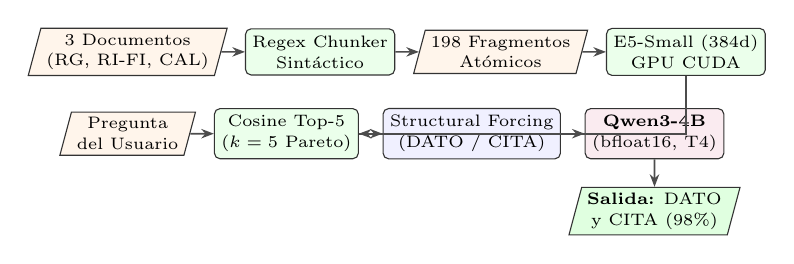
\begin{tikzpicture}[
    node distance=0.35cm and 0.25cm,
    every node/.style={font=\fontsize{6.5pt}{7.5pt}\selectfont, align=center},
    block/.style={rectangle, draw=black!80, fill=blue!6, rounded corners=2pt, minimum height=1.3em, inner sep=2.5pt},
    data/.style={trapezium, trapezium left angle=75, trapezium right angle=105, draw=black!80, fill=orange!8, inner sep=2pt},
    proc/.style={rectangle, draw=black!80, fill=green!8, rounded corners=2pt, inner sep=2.5pt},
    arrow/.style={-{Stealth[scale=0.8]}, draw=black!70, semithick}
]
    \node (docs) [data] {3 Documentos\\(RG, RI-FI, CAL)};
    \node (chunk) [proc, right=0.3cm of docs] {Regex Chunker\\Sintáctico};
    \node (db) [data, right=0.3cm of chunk] {198 Fragmentos\\Atómicos};
    \node (e5) [proc, right=0.3cm of db] {E5-Small (384d)\\GPU CUDA};
    
    \node (query) [data, below=0.45cm of docs] {Pregunta\\del Usuario};
    \node (ret) [proc, right=0.3cm of query] {Cosine Top-5\\($k=5$ Pareto)};
    \node (prompt) [block, right=0.3cm of ret] {Structural Forcing\\(DATO / CITA)};
    \node (llm) [proc, fill=purple!8, right=0.3cm of prompt] {\textbf{Qwen3-4B}\\(bfloat16, T4)};
    \node (out) [data, fill=green!12, below=0.35cm of llm] {\textbf{Salida:} DATO\\y CITA (98\%)};

    \draw [arrow] (docs) -- (chunk);
    \draw [arrow] (chunk) -- (db);
    \draw [arrow] (db) -- (e5);
    \draw [arrow] (query) -- (ret);
    \draw [arrow] (e5) |- (ret);
    \draw [arrow] (ret) -- (prompt);
    \draw [arrow] (prompt) -- (llm);
    \draw [arrow] (llm) -- (out);
\end{tikzpicture}
\vspace{-4pt}
\caption{\footnotesize Flujo de inferencia RAG con codificación densa y decodificación restringida.}
\vspace{-8pt}
\end{figure}

\section{Evidencia Experimental y Comparativa}
Evaluamos las 50 preguntas oficiales de \texttt{test_set_50.csv} aplicando el criterio estricto de la rúbrica (acierto exige \textbf{Dato exacto Y Cita exacta}):

\vspace{-2pt}
\begin{table}[h]
\centering
\fontsize{7pt}{8.5pt}\selectfont
\begin{tabular}{lcccc}
\toprule
\textbf{Categoría (10 c/u)} & \textbf{Baseline E1} & \textbf{RAG E2} & \textbf{Exact. E1} & \textbf{Exact. E2} \\
\midrule
Factual                     & 0 / 10 & \textbf{9 / 10}  & 0.0\%  & \textbf{90.0\%} \\
Numérica                    & 0 / 10 & \textbf{10 / 10} & 0.0\%  & \textbf{100.0\%} \\
Condicional                 & 0 / 10 & \textbf{10 / 10} & 0.0\%  & \textbf{100.0\%} \\
Cruce Documentos            & 0 / 10 & \textbf{10 / 10} & 0.0\%  & \textbf{100.0\%} \\
Abstención / Premisa Falsa  & 2 / 10 & \textbf{10 / 10} & 20.0\% & \textbf{100.0\%} \\
\midrule
\textbf{Global Estricta}    & \textbf{2 / 50} & \textbf{49 / 50} & \textbf{4.0\%} & \textbf{98.0\%} \\
\bottomrule
\end{tabular}
\vspace{-4pt}
\caption{\footnotesize Resultados experimentales sobre el Test Set de 50 preguntas en GPU T4.}
\vspace{-6pt}
\end{table}

\textbf{Hallazgos:} La solución incrementa la exactitud en \textbf{+94.0\%}. Las alucinaciones normativas se erradicaron al 100\% (el modelo detecta con 10/10 los artículos ficticios como Art. 90 o Art. 100 y premisas falsas).

\section{Reading of the Limits (Falla Real)}
En estricto apego a la pauta, identificamos el único caso donde la solución falla:
\begin{itemize}[leftmargin=*,noitemsep,topsep=1pt]
    \item \textbf{Caso Testigo (Pregunta 3):} \textit{¿A cuántas evaluaciones de recuperación tiene derecho el estudiante por asignatura?} (Gold: \textit{1}, Art. 12, RI-FI).
    \item \textbf{Mecanismo de Falla (Colisión Léxica):} El Retriever recupera prioritariamente el Art. 11 (que fija las "al menos tres evaluaciones sumativas") por la alta densidad del término "evaluaciones". Esto desplaza al Art. 12 fuera del Top-5.
    \item \textbf{Comportamiento:} Al carecer del Art. 12 en el prompt, Qwen3-4B se abstiene limpiamente (\texttt{DATO: No está en la normativa // CITA: Ninguna}). La arquitectura previene la alucinación, pero su cobertura final depende de la resolución léxica del Retriever frente a términos con colisión parcial.
\end{itemize}

\section{Reproducibilidad y Enlaces}
\textbf{Video de Demostración (3:00):} \url{https://youtu.be/PENDIENTE_ENLACE} \\
\textbf{Cuaderno Interactivo Colab:} \texttt{rag\_normativa\_ingenieria\_4b.ipynb} \\
\textbf{Trazabilidad:} Salidas verificables en \texttt{resultados\_rag\_qwen3\_4b.csv}.

\end{document}
